Der Aufbau einer PST-Datei ist in Abbildung \ref{fig:pstarchitecture} abgebildet. Er besteht aus drei Schichten:

\begin{itemize}
    \item Messaging Layer
    \item LTP Layer (Lists, Tables, and Properties)
    \item NDB Layer (Node Database)

\end{itemize}

Aus der Dokumentation des .pst-Dateiformats kann folgendes entnommen werden: \newline
Die Messaging Layer besteht aus den übergeordneten Regeln und der Geschäftslogik, die es ermöglichen, die Strukturen der LTP- und NDB-Schichten zu kombinieren und als Ordnerobjekte, Nachrichtenobjekte, Attachment-Objekte und Eigenschaften zu interpretieren. Die Messaging-Schicht definiert auch die Regeln und Anforderungen, die beim Ändern des Inhalts einer PST-Datei befolgt werden müssen, damit die geänderte PST-Datei weiterhin erfolgreich von Implementierungen dieses Dateiformats gelesen werden kann. \newline
Die LTP-Schicht implementiert übergeordnete Konzepte auf dem NDB-Konstrukt. Die Kernelemente der LTP-Schicht sind der Property Context (PC) und der Table Context (TC). Ein PC repräsentiert eine Sammlung von Eigenschaften. Ein TC stellt eine zweidimensionale Tabelle dar. Die Zeilen stellen eine Sammlung von Eigenschaften dar. Die Spalten geben an, welche Eigenschaften in den Zeilen enthalten sind.
Vom Standpunkt einer High-Level-Implementierung aus gesehen, wird jeder PC oder TC als Daten in einem einzelnen Knoten gespeichert. Die LTP-Schicht verwendet NIDs, um PCs und TCs zu identifizieren.\newline
Um PCs und TCs effizient zu implementieren, verwendet die LTP-Schicht die folgenden zwei Arten von Datenstrukturen über jedem NDB-Knoten.
Die NDB-Schicht besteht aus einer Datenbank von Knoten, die die untergeordneten Speichermöglichkeiten des PST-Dateiformats darstellt. Aus der Sicht der Implementierung besteht die NDB-Schicht aus dem Header, den Dateizuordnungsinformationen, Blöcken, Knoten und zwei BTrees: dem Node BTree (NBT) und dem Block BTree (BBT). Der NBT enthält Verweise auf alle zugänglichen Knoten in der PST-Datei. Seine BTree-Implementierung ermöglicht eine effiziente Suche nach einem bestimmten Knoten. Jeder Knotenverweis wird durch einen Satz von vier Eigenschaften dargestellt, die seine NID, übergeordnete NID, Daten-BID und Unterknoten-BID umfassen. Die Daten-BID verweist auf den Block, der die mit dem Knoten verbundenen Daten enthält, und die Unterknoten-BID verweist auf den Block, der Verweise auf Unterknoten dieses Knotens enthält. Die NIDs der obersten Ebene sind im gesamten PST eindeutig und können von der NBT aus durchsucht werden. Unterknoten-NIDs sind nur innerhalb eines Knotens eindeutig und können nicht über die NBT gesucht (oder gefunden) werden. Die übergeordnete NID ist eine Optimierung für die höheren Schichten und hat keine Bedeutung für die NDB-Schicht. Der BBT enthält Verweise auf alle Datenblöcke der PST-Datei. Seine BTree-Implementierung ermöglicht eine effiziente Suche nach einem bestimmten Block. Ein Blockverweis wird durch einen Satz von vier Eigenschaften dargestellt, zu denen seine BID, IB, CB und CREF gehören. IB ist der Offset innerhalb der Datei, an dem sich der Block befindet. CB ist die Anzahl der im Block gespeicherten Bytes. CREF ist die Anzahl der Verweise auf die im Block gespeicherten Daten. Auf die Wurzeln der NBT und BBT kann über den Header der PST-Datei zugegriffen werden.
Das folgende Diagramm \ref{fig:nodesblockspst} veranschaulicht die Beziehung zwischen Knoten und Blöcken auf hoher Ebene \cite{.c}.

\begin{figure}
    \centering
    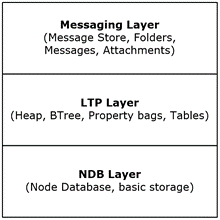
\includegraphics[width=0.50\textwidth]{images/PST_File.png}
    \caption{Logische Architektur einer PST-Datei \cite{.c}} 
    \label{fig:pstarchitecture}
\end{figure}

\begin{figure}
    \centering
    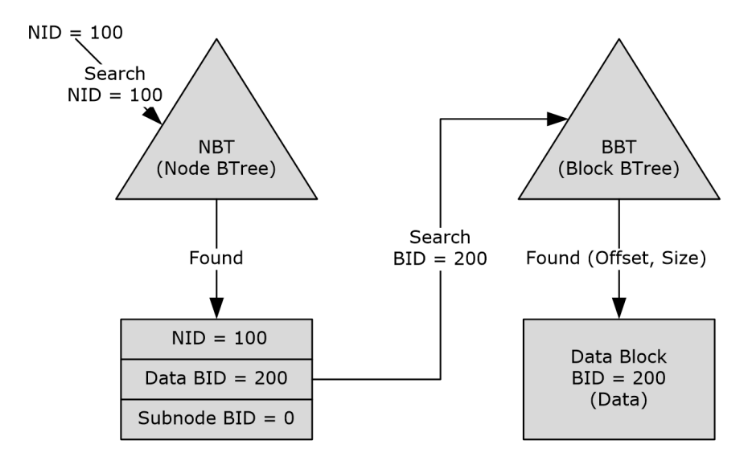
\includegraphics[width=0.75\textwidth]{images/nodes_blocks_pst.PNG}
    \caption{Beziehung zwischen Knoten und Blöcken \cite{.c}} 
    \label{fig:nodesblockspst}
\end{figure}